\section{Experiments}
Our experiments were conducted using 9600 entries generated from the PROXIMITY DBLP database of Computer Science bibliographies \cite{DBLP}.  Each bibliographic sequence contains 8 fields pertaining to the title, authors, conference, ISBN, publisher, volume, proceedings, and year.  Training was performed on 4600 entries and testing on 5000 entries.  We implemented most of the CrowdPillar algorithm in Java 1.8 using the feature set provided by Sarawagi \cite{Sarawagi04}.
\begin{figure}
\centering
\subfigure[Correctly Labeled]{\label{fig:blue}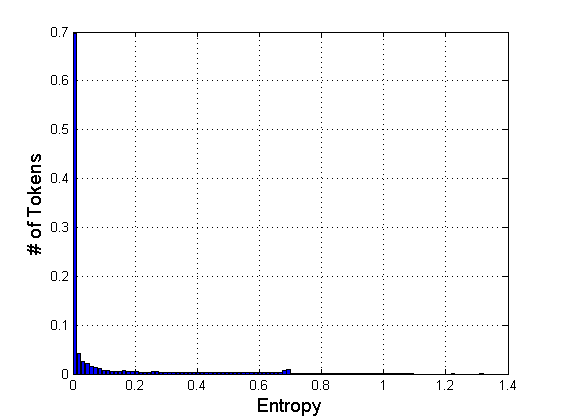
\includegraphics[width=0.35\textwidth]{images/blue.png}}
\subfigure[Incorrectly Labeled]{\label{fig:red}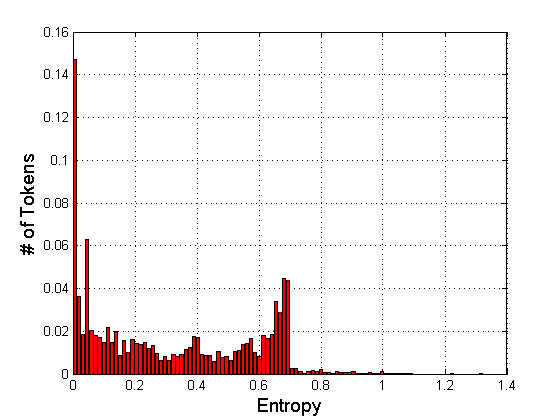
\includegraphics[width=0.35\textwidth]{images/red.png}}
\caption[example] {Normalized entropy histograms for correctly and incorrectly labeled tokens.}
\end{figure} 

\subsection{Entropy vs. Inaccuracy}
The fundamental assumption our question formulation methods hinge upon is the direct correlation between inaccurate tokens and their marginal entropy level.  Figures \ref{fig:blue} and \ref{fig:red} demonstrate the veracity of this assumption.  The marginal entropy of every token in the 5000 sequence test set is measured and histogrammed by correct and incorrect sequences. The majority of accurate tokens tend to lower entropy values while the inaccurate ones appear in a much higher range.

\subsection{Uncertainty Reduction}
It is intractable to be able to ask a question about every node and send it to the crowd.  The key to CrowdPillar's success is the ability to optimally select nodes from budget size of $k$ sequences which reduce uncertainty in the entire system the most.  In testing our node selection algorithm, the chosen nodes were replaced by their ground truth values.  In practice, as discussed in Section 5, the real feedback from the crowd is complex and probabilistic.  After being clamped to the nodes' ground truth values, each sequence was re-run with Constrained Viterbi to produce a new label sequence.

\begin{figure}
\centering
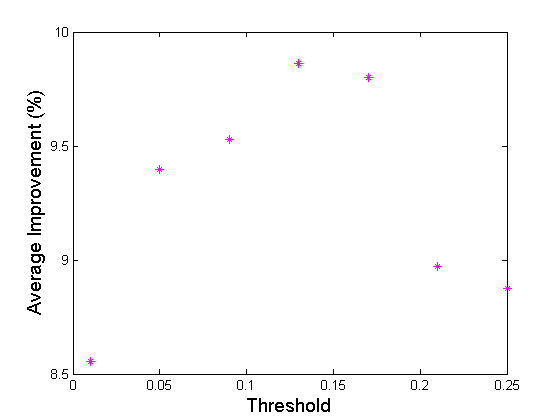
\includegraphics[width=0.48\textwidth]{images/threshold.png}
\caption[example] { 
\label{fig:thresh} 
Average increase in accuracy for each clamped sequence selected by various thresholds.  The threshold determines the level above which a node's entropy is considered "high".}
\end{figure} 

In practice, it is impractical to select a node from every sequence for sending to the crowd, so we sort the sequences according to some metric and select the top $k$ depending on the budget.  We tested two different sorting metrics.  The first takes sorts by the entropy of the maximum entropy node in the sequence.  The second is slightly more complex.  We classified each sequence by the number of "high" entropy nodes it contained.  The threshold for determining what constituted high entropy was found by a parameter search.  Figure \ref{fig:thresh} shows the average increase in accuracy for the top 500 testing sequences sorted by the number of high entropy nodes determined by each threshold.  Based on the results, we deduced $\tau=0.13$ as an appropriate threshold.

After determining which sequences needed to be corrected by the two sorting metrics, we tested two different methods of assigning scores to each node as discussed in Section 4.  We either assigned $S_{t}$ to be the marginal entropy or the neighborhood marginal entropy with neighborhoods including tokens before and after node $t$.

\begin{figure}
\centering
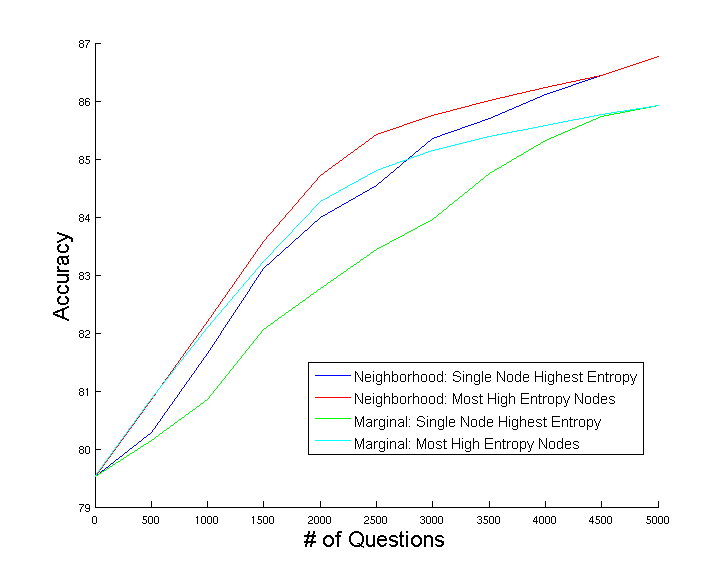
\includegraphics[width=0.5\textwidth]{images/budget.png}
\label{fig:budget}
\caption[example]{Comparison of the 4 different methods for sorting sequences and scoring nodes within each sequence.}
\end{figure}

The two sorting metrics and two scoring metrics allowed for four distinct ways of selecting the top $k$ sequences and then selecting a node from those sequences.  Figure \ref{fig:budget} shows the accuracy increase for each of these methods as a function of the number of questions asked.  Sorting by the number of high entropy nodes appears to be the best metric for determining inaccurate sequences.  The neighborhood marginal entropy as a scoring metric also provides a small boost compared to simply taking the single node's marginal entropy.  The combination of neighborhood marginal and number of high entropy nodes produced as much as a 7\% total increase in accuracy when applied to all questions in the testing set.

\subsection{Dempster-Shafer Combination}

\begin{figure}
\centering
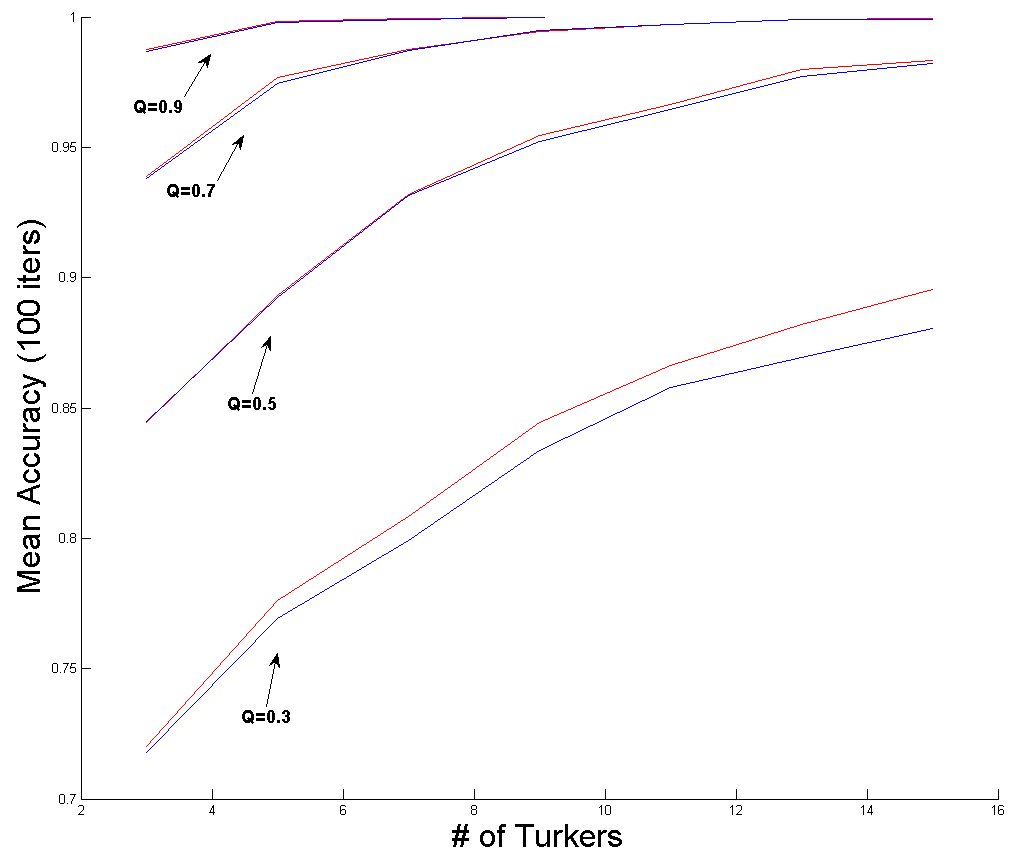
\includegraphics[width=0.425\textwidth]{images/DS_fixed.png}
\caption[example] { 
\label{fig:DS} 
Comparison of Dempster-Shafer combination (red) vs. majority voting (blue) for possibly unreliable Turkers.  Q denotes the mean quality level of the selected Turkers.  The DS method increases in performance compared to majority voting as the Turkers become more unreliable.}
\end{figure} 

To test the use of DS combination vs. majority voting for probabilistic data, we generated a synthetic data set for Turker responses to 1,000 binary questions.  $M$ Turker responses were generated for each question for a total of $1000M$ responses, where $M = $3, 5, 7, 9, 11, and 15.  For each response, a Turker was generated with quality rating drawn from a normal distribution centered at 0.9, 0.7, 0.5, and 0.3 with a deviation of 0.1 and thresholded beteen [0,1].  The quality rating determined the likelihood that Turker's answer reflected the ground truth.  For example, a Turker with a quality rating of 0.7 was associated with an answer that was correct with 70\% probability and a random choice with 30\% probability.  This rating could be derived from the individual Turker quality or could be seen as a function of a difficult question that produces low quality results.

Figure \ref{fig:DS} shows an accuracy comparison between Dempster-Shafer combined responses and those combined with majority voting for differing levels of Turker quality.  It's observed that the poorer the quality of the Turker or the question, the worse majority voting does in relation to DS.  DS obtains it's full power when the quality of responses is very poor and there exists a large uncertainty between answers.
